\subsection{Do Evolved Skills Remain Useful When Tasks Change?}
\label{sec:variant-transfer}

A source-task skill may capture a reusable procedure, a decision rule, or assumptions specific to that instance. We deploy these skills on controlled variants while keeping each artifact frozen (Figure~\ref{fig:variant-evaluation}). The executor interprets the changed task and decides how to use the existing skill. Its reward difference from a no-skill execution of the same variant measures the final artifact's utility under that change.

\paragraph{Three forms of task change.}
Input-representation changes (P1) alter how the task is presented, including names, column arrangements, or schemas. They test whether the executor can recover the relevant roles of the inputs while using the skill. Task-instance changes (P2) replace the data or instance structure. They test whether the procedure can be instantiated with new values rather than relying on a solution specific to the source instance. Coupled-requirement changes (P3) alter or add requirements that must be handled together. They test whether the executor can adapt the procedure while preserving the constraints that determine a valid output. These changes probe different aspects of reuse rather than successive levels of difficulty.

The record contains 222 task variants and 886 condition-level results across no skill and the three methods. Table~\ref{tab:variant-transfer} summarizes historical and recovery evaluations for 222 SkillEvolver variants and 221 each for SPARK and CoEvoSkills. Panel B separates the within-variant differences by type of change.

\paragraph{Overall utility under task variation.}
SkillEvolver increases mean reward from 41.87 to 53.81, a gain of 11.94 points, with 47 improved and 20 regressed variants. Thus, its source-task skills retain positive average utility after the tasks change. SPARK increases mean reward from 41.61 to 42.25, a gain of 0.65 points, with 32 improvements and 37 regressions. The positive mean alongside more regressions than improvements reflects the magnitudes of the reward changes: the mean and the number of benefited variants capture different properties. CoEvoSkills decreases mean reward from 41.61 to 36.60, a change of $-5.01$ points, with 26 improvements and 41 regressions. Its positive source-task gains therefore coexist with negative average utility on the recorded variants.

\paragraph{Where does utility extend?}
SkillEvolver has positive gains under every type of change: 11.85 points on P1, 14.56 on P2, and 9.72 on P3. Improved variants also outnumber regressed variants within each type: 15 versus seven, 15 versus six, and 17 versus seven, respectively. Its overall gain consequently spans all three forms of variation. The largest mean gain occurs under P2, where applying the source skill requires working with a changed instance.

The other methods exhibit different profiles. SPARK remains positive on P1 and P3, at 2.00 and 4.53 points, but falls by 5.23 points on P2. CoEvoSkills has negative average changes on all three types, with its largest decline also on P2 ($-9.51$ points, compared with $-3.59$ on P1 and $-2.42$ on P3). Instance changes thus separate the observed reuse profiles especially clearly: SkillEvolver's largest positive gain and the other methods' largest declines occur in the same category of variation.

\paragraph{What the combined results reveal.}
All three methods obtain positive mean gains in both standard-task runs, yet their variant profiles differ substantially. Success on the source tasks and usefulness after task changes are distinct empirical properties. SkillEvolver provides the clearest positive reuse pattern in these records, whereas SPARK's benefit depends on the type of change and CoEvoSkills' source-task benefit does not extend on average. Approximately seven in ten variants remain tied with the baseline for each method. The gains therefore arise from a subset of changed outcomes, motivating a closer examination of the decisions expressed when a skill helps or hinders execution.

\begin{figure*}[t]
\centering
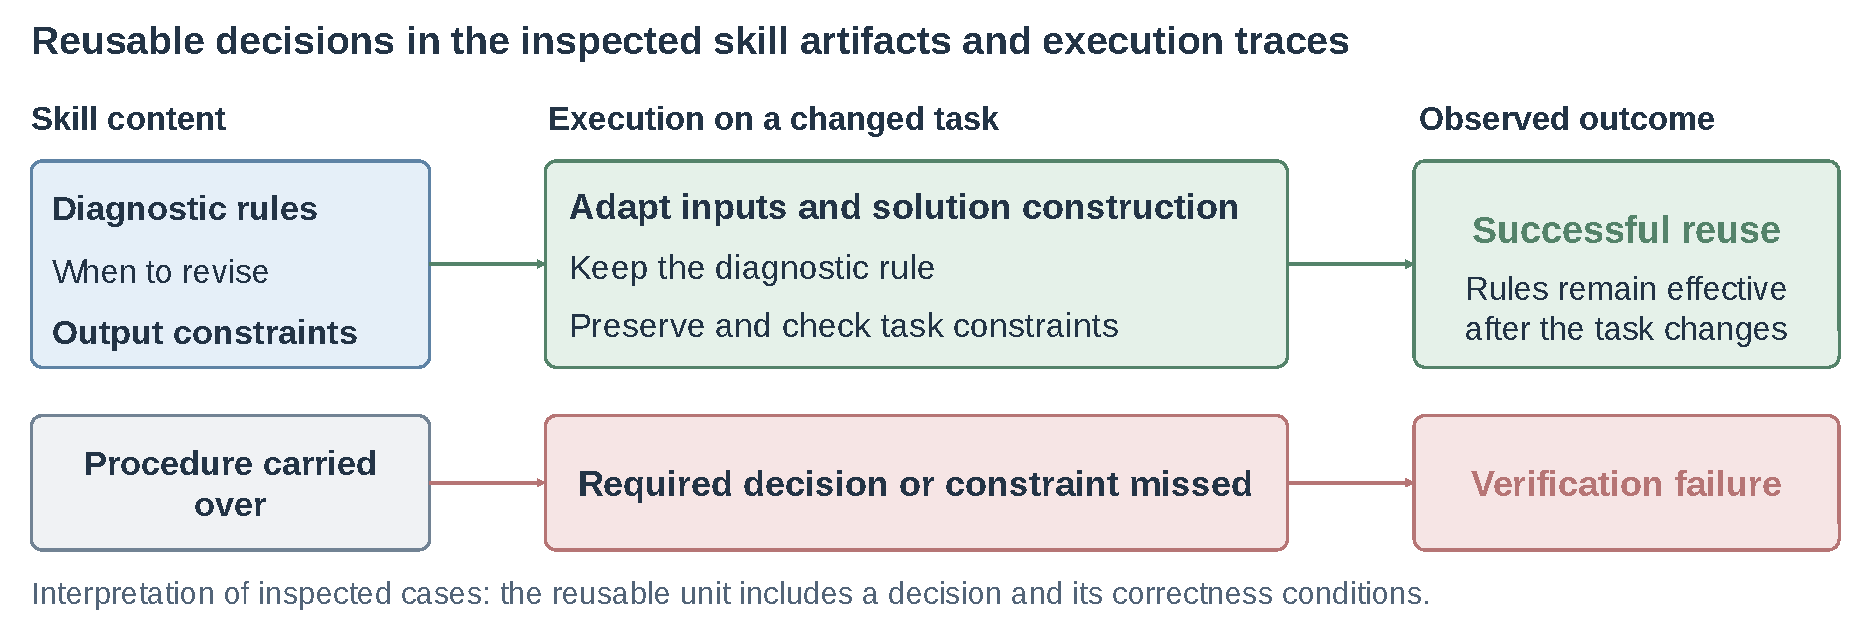
\includegraphics[width=\textwidth]{figures/skill-reuse-logic.pdf}
\caption{Skill reuse in the inspected cases. Diagnostic rules guide adaptation, and correctness constraints guide output checks. Successful reuse preserves these decisions while adapting the solution; unsuccessful reuse can carry over a procedure while missing a required decision or constraint.}
\label{fig:skill-reuse}
\end{figure*}

\subsection{What Is Preserved When a Skill Is Reused?}
\label{sec:skill-reuse}

To interpret the variant results, we inspect the skill artifacts together with their execution traces. We distinguish the procedure stored in a skill from the way an executor applies it to a new task. A script can preserve an action sequence, while successful reuse also depends on recognizing when that sequence applies, adjusting its inputs, and checking its output. Figure~\ref{fig:skill-reuse} organizes the inspected evidence around these decisions.

\paragraph{Diagnostic rules guide adaptation.}
In the inspected SkillEvolver artifacts, intermediate checks guide the choice and revision of a procedure. Candidate discovery, diagnosis, and refinement appear as separate operations, with conditions explaining when to revisit an intermediate result. This structure gives the executor opportunities to respond to changed inputs before committing to an output. In the signal-detection traces, for example, the executor uses diagnostic checks to distinguish competing candidate explanations and adjusts the search accordingly. The reusable content is the rule for evaluating a candidate; the candidate values and search settings can change with the task.

\paragraph{Correctness constraints survive solution changes.}
A second form of reusable content specifies which properties the output must preserve. The inspected scheduling skill expresses constraints relative to the supplied instance and baseline, allowing the executor to construct a different schedule while checking the same repair requirements. Failure traces make this distinction visible: much of a workflow can execute correctly while one omitted requirement invalidates the final result. This helps explain why preserving a familiar procedure is insufficient when a variant changes how inputs are represented or how requirements interact.

\paragraph{Reuse combines preserved rules with new execution.}
Across the inspected cases, successful adaptation preserves decision criteria and correctness checks while changing input handling, search choices, or the constructed solution. This illustrates how a transferred artifact can help the executor decide what to retain and what to recompute. SkillEvolver's positive profile across P1--P3 is consistent with this form of reuse. The trace evidence identifies concrete instances of that behavior. Complementary interventions on SkillRevise, SkillHone, and SkillOpt later in the paper test component effects within their respective artifact lineages.

The variant evaluations characterize how far final-skill utility extends beyond the source task. The following retention and lifecycle studies examine whether improvements persist under fresh deployment and which parts of the evolution process produce them.
